% 导言区
\documentclass{article}
%\documentclass{paper}
\usepackage{pythonhighlight}

\usepackage{ctex}
\usepackage{amsmath}
\usepackage{graphicx}
\usepackage{bbding}
\usepackage{multirow}
\usepackage{listings}
\usepackage{amssymb}


\graphicspath{{figs/}}

\title{\heiti 第二次作业}
\author{\kaishu 宋晓宇}
\date{}
\newcommand{\bs}{\boldsymbol}
\newcommand{\p}[1]{\includegraphics[width=0.7\textwidth]{#1}}

% 正文区(文稿区)
\begin{document}
	\maketitle
	\section*{1.}

	运行结果:最小值点:$ [-1.   1.5] $,最小值:$-1.25$,迭代次数: $2$.
	
    \section*{2.}
	
    结果如下:

    Golden Section Search 
    
    Minimum value: -1.125 at 0.257 - iterations : 8

    Fibonacci Search 
    
    Minimum value: -1.125 at 0.265 - iterations : 7

    Bisection Search
    
    Minimum value: -1.124 at 0.234 - iterations : 6

    Dichotomous Search 
    
    Minimum value: -1.125 at 0.254 - iterations : 7

    Shubert-Piyavskii 
    
    Minimum value: -0.97 at -0.028 - iterations : 3

    Golden Section Search 
    
    Minimum value: -39.88 at 3.609 - iterations : 12
    
    Fibonacci Search 
    
    Minimum value: -39.879 at 3.614 - iterations : 12

Bisection Search

Minimum value: -39.88 at 3.589 - iterations : 9

Dichotomous Search 

Minimum value: -39.88 at 3.591 - iterations : 10

Shubert-Piyavskii 

Minimum value: -1.0 at 0 - iterations : 1


    \section*{3}

    运行结果如下:

    Goldstein 
    
    alpha:1.0 - iterations : 20

Goldstein-Price 

alpha:0.0 - iterations : 8

Wolfe-Powell 

alpha:0.0 - iterations : 8



	\section*{4.}
	
    \subsection*{a)}

	$f(x_1, x_2, x_3) = max(|x_1|, |x_2|, |x_3|)$, 在点$(0,0,0)$处. 由次梯度定义$\partial f = {g | g^t(y-x) \le f(y)-f(x)} \forall y \in \mathbf{dom} f$,
	\begin{align*}
		f(\mathbf{x}) &\ge f(\mathbf{0})+ \mathbf{g^t} \mathbf{x} \\
		\max \{ |\mathbf{x}| \} &\ge 0 + \mathbf{g^t} \mathbf{x}  \\
		\max \{ |\mathbf{x}| \} &\ge  \mathbf{g^t} \mathbf{x} 
	\end{align*}
	
	故有:$|| g||_1 \le \mathbf{1}$

    \subsection*{b)}

	\begin{equation*}
		f(x) \ge f(0) + gx \leftarrow
		\begin{cases}
			x>0 \quad \quad g < \frac{e^x -1 }{x} \quad s.t. g< \lim_{x \to 0^+}\frac{e^x -1 }{x}  = 1\\
			x<0 \quad \quad g > \frac{e^{-x} -1 }{x} \quad s.t. g> \lim_{x \to 0^-}\frac{e^{-x} -1 }{x} = -1 \\
		\end{cases} 
	\end{equation*}

	所以次梯度g = $[-1,1]$.

    \subsection*{c)}

    $f(x_1, x_2) = max (x_1+x_2-1, x_1-x_2+1)$, 在点$(1,1)$处,
    由次梯度基本运算法则和逐点最大值性质可得:
    \begin{gather*}
        \partial f = conv \cup_{i \in I(x)} \partial f_i(x) \\
        \partial f_1(x) = A_1 , \quad A_1 = (1, 1)^T \\
        \partial f_2(x) = A_2 , \quad A_2 = (1, -1)^T \\
    \end{gather*}
    
    \section*{5.}

	最小值点为$(0,0)$,最小值为0.

    \section*{6.}

	最小值点为$(2,1)$,最小值为-8.
    
    \section*{7.}

    运行结果如下:

    DFP 
    
    Minimum value: -1.25 at [-1.   1.5] - iterations : 2

    BFGS 

    Minimum value: -1.25 at [-1.   1.5] - iterations : 2

    FR 
    
    Minimum value: -1.25 at [-1.   1.5] - iterations : 2

    DFP法和BFGS法都是拟牛顿法,主要是为了解决牛顿法中Hesse逆矩阵不可解的问题
    拟牛顿法需要较大存储空间,求解大型问题可能会遇到困难。
    和拟牛顿法相比,共轭方向法的优点在于存储量较小, 在求解大型优化问题时占优势。 

    \section*{8.}

    \subsection*{梯度下降法的收敛性}
    
    梯度下降法的基本思想是沿着负梯度方向更新参数,以找到函数的局部最小值。假设我们有一个可微的目标函数 $f: \mathbb{R}^n \to \mathbb{R}$,其梯度为 $\nabla f(x)$,并且假设它是Lipschitz 连续的,即存在常数 $L > 0$,使得:\[ \|\nabla f(x) - \nabla f(y)\| \leq L \|x - y\| \quad \forall x, y \in \mathbb{R}^n \]

    \subsubsection*{收敛性证明}

    1. \textbf{更新规则}:
    \[ x_{k+1} = x_k - \alpha_k \nabla f(x_k) \]
    其中 $\alpha_k$ 是步长。

    2. \textbf{函数值下降}:
    利用泰勒展开:
   \[
   f(x_{k+1}) \leq f(x_k) + \nabla f(x_k)^T (x_{k+1} - x_k) + \frac{L}{2} \|x_{k+1} - x_k\|^2
   \]
   代入更新规则后,得到:
   \[
   f(x_{k+1}) \leq f(x_k) - \alpha_k \|\nabla f(x_k)\|^2 + \frac{L \alpha_k^2}{2} \|\nabla f(x_k)\|^2
   \]

3. \textbf{选择合适的步长}:
   选择 $\alpha_k$ 满足 $0 < \alpha_k < \frac{1}{L}$,则可以证明:
   \[
   f(x_{k+1}) < f(x_k)
   \]
   这表明梯度下降法在每一步都能减少目标函数的值。

4. \textbf{收敛性}:
   通过对函数值的递减性和有界性,可以得出梯度下降法在适当条件下是收敛的。

\subsection*{牛顿法的收敛性}

牛顿法利用二阶导数信息来加速收敛,主要用于优化目标函数。

\subsubsection*{收敛性证明}

1. \textbf{更新规则}:
   \[
   x_{k+1} = x_k - H^{-1} \nabla f(x_k)
   \]
   其中 $H$ 是目标函数的海森矩阵。

2. \textbf{局部收敛性}:
   若 $x^*$ 是 $f$ 的局部极小点,且 $H$ 在 $x^*$ 处是正定的,则牛顿法在 $x$ 足够接近 $x^*$ 时具有二次收敛性。

3. \textbf{函数值的下降}:
   通过泰勒展开和海森矩阵的性质,可以证明牛顿法的收敛速度比梯度下降法快。

\subsection*{二次规划问题的收敛性分析}

考虑二次规划问题:
\[
\min \frac{1}{2} x^T Q x + c^T x
\]
其中 $Q$ 是正定矩阵。

1. \textbf{梯度和海森矩阵}:
   \[
   \nabla f(x) = Qx + c
   \]
   \[
   H = Q
   \]

2. \textbf{收敛性分析}:
   - \textbf{梯度下降法}:利用上述收敛性证明,对于二次目标函数,选择合适的步长 $\alpha_k$ 后,函数值会逐步减小,最终收敛至最优解。
   - \textbf{牛顿法}:因为 $Q$ 是正定的,牛顿法会在每一步快速收敛到最优解。

    \subsection*{结论}

    梯度下降法和牛顿法在适当条件下都具有收敛性。对于二次规划问题,利用梯度法可以有效地达到最优解,且牛顿法通常收敛更快。通过选择合适的步长和利用二阶信息,可以加速收敛过程。

    \section*{9}

    无约束优化问题的基本目标是寻找一个变量集合 $x \in \mathbb{R}^n$,使得目标函数 $f(x)$ 达到最小值。无约束优化的基本思想可以概述为以下几个步骤:

    1. \textbf{目标函数的选择}:选择一个需要优化的目标函数 $f(x)$,该函数通常需要满足可微性条件,以便计算其梯度和海森矩阵。

    2. \textbf{初始点的选择}:选择一个合适的初始点 $x_0$,为优化算法提供起始位置。

    3. \textbf{迭代更新}:利用梯度信息或二阶导数信息,采用优化算法(如梯度下降法、牛顿法等)逐步更新解的值,直到满足收敛条件。

    4. \textbf{收敛性检查}:根据设定的收敛标准(如梯度范数、函数值变化等)判断是否达到最优解,若未达到,则继续迭代。

    无约束优化问题的求解,分为两大类算法:
    \begin{itemize}
        \item \textbf{利用导数信息}的算法,包括最速下降法,牛顿法,共轭梯度法,拟牛顿法。
    这类方法是利用梯度信息,来选取合适的搜索方向,搜索方向要要满足使得函数值下降的要求。
        \item  \textbf{不利用导数信息}的\textbf{直接优化方法},包括模式搜索、Powell方法、Rosenbrock法、单纯形搜索等,实际上是根据规则在空间中挑选线性无关的搜索方向,自然地,这类方法对于求解变量不多的优化问题比较有效。
    \end{itemize}
    
    一般而言,无约束优化问题的求解涉及两个关键的问题,一个是确定当前点的搜索方向,二是确定搜索步长。

    \subsection*{如何将非凸优化问题转化成凸优化问题}

    首先需要说明相比于非凸问题,凸问题的优势。
    对于凸问题,局部最优解就是全局最优解(更准确的说法是严格凸函数),同时,非凸问题的困难在于在高维空间中,存在许多鞍点(梯度为零,但是
    Hesse矩阵不定)。

    回顾凸问题的定义,需要满足两个条件(1)问题的可行域是一个凸集;(2)目标函数是可行域上的一个凸函数。

    在非凸问题转化成凸问题的过程中可以从这两个方向入手:
    \begin{itemize}
        \item 修改目标函数,使其成为一个凸函数,这样就可以满足条件(1)。
        \item 抛弃一些约束条件,或者对约束条件做松弛处理,使得新的可行域是凸集,同时包含原可行域的所有点。
    \end{itemize}

	\subsection*{如何将有约束问题转化成无约束优化问题}

    将针对可行域的约束条件作为惩罚项加入原目标函数,比如常见的罚函数方法(内点法,外点法);同时为了解决罚函数方法中的缺陷,可采用增广拉格朗日方法。

	\section*{10.}

	统一公式描述:

    \begin{equation*}
        x^{k+1} = x^{k} - \lambda_k d^{k}
    \end{equation*}

    其中,$\lambda_k$ 是每次迭代的步长,$d^{(k)}$ 是每次迭代的搜索方向。
    对于上述方法:

    \begin{itemize}
        \item 最速下降法: 搜索方向是$-\nabla f(x^k)$,可以通过方向导数来证明负梯度是在$x^k$点局部下降最快的方向
        (并非全局下降最快的方向), 每次迭代步长可以通过一维搜索方法确定最优的$\lambda_k$。
        \item 牛顿法: 搜索方向是$-\nabla^2 f(x^k)^{-1} \nabla f(x^k)$, 每次迭代步长为1。牛顿法的基本思想是$x^k$点附近用
        二阶的泰勒展开,用二次函数的极值点近似目标函数的极值点,但是如果$x^k$不满足前提,搜索方向不能保证是下降方向。
        \item 修正牛顿法:牛顿法存在的问题是Hesse的逆矩阵不一定可解,且迭代步长为定值。修正牛顿法的思想是(1)修正Hesse矩阵为
        $B_k = \nabla^2f(x^k) + \epsilon I$,同时用一维搜索方法确定最优的$\lambda_k$。
    \end{itemize}

    \subsection*{变尺度法的基本思想:}

    和修正牛顿法不同,变尺度法通过秩2近似,直接求解Hesse矩阵的逆矩阵的近似矩阵$H_k$, 使得近似矩阵$H_k$满足拟牛顿条件
    然后用一维搜索算法确定搜索步长。
    \begin{align*}
        p^k &= x^{k+1}- x^{k} \\
        q^k &= g^{k+1}- g^{k} \\
        p^k &= H_{k+1}q^k \\ 
    \end{align*}

	\section*{11.}

    
    选取第6题中的优化问题,选择用带有动量的梯度下降优化,运行结果如下:

    最小值点: [-2   1]
    
    最小值: -8.0
    
    迭代次数: 115

	\section*{12.}

    参数变化符合低维特性,如图:

    \begin{figure}[h!]
        \centering
        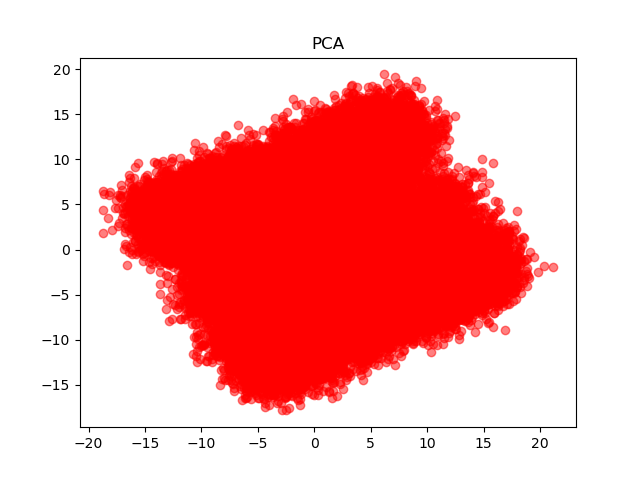
\includegraphics[width=0.5\linewidth]{./figs/PCA.png}
        \caption{ResNet-18 activations-PCA}
        \label{fig:pca}
    \end{figure}

    \begin{figure}[h!]
        \centering
        
\includegraphics[width=0.5\linewidth]{./figs/tsne.png}
        \caption{ResNet-18 activations-t-SNE}
        \label{fig:tsne}
    \end{figure}


	\section*{13.}

	一阶优化算法的最新加速思想主要有如下几种:

	随机梯度法:在每次迭代中,随机选择一个样本点来计算梯度,避免了计算所有样本点的梯度,节省了计算时间。

	动量加速法:考虑最速下降法在由于相邻两次的搜索方向正交,导致在最优点附近出现zig-zag现象。考虑用利用上一步的梯度信息加速收敛。
    
	Nesterov动量加速:在每次迭代中,考虑上一次的梯度信息,来加速当前的搜索方向。

    \section*{14.}

    \subsection*{Krylov方法的基本思想}

    Krylov方法的核心在于:

    利用矩阵-向量乘积:通过不断计算矩阵与向量的乘积,生成一组基底向量,构建Krylov子空间。

    投影到低维子空间:将原始高维问题投影到低维的Krylov子空间上,转化为一个小规模的子问题(如小矩阵的特征值或线性方程组)。

    迭代优化:在子空间中寻找最优近似解,例如使残差最小化,或满足某种正交性条件(如Ritz-Galerkin条件)。

    \subsection*{子空间投影的典型应用}

    1. 线性方程组求解:求解大型稀疏线性方程组 ,常见于物理建模(如流体力学、电磁场仿真)和离散化偏微分方程(PDE)问题。

    2. 特征值问题:计算大型矩阵的少数极端特征值(如最大或最小模)及其对应特征向量,常见于振动分析、量子力学和主成分分析(PCA)。

    3. 模型降阶(Model Order Reduction, MOR):简化高维动力系统模型(如微电子器件、控制系统),保留关键动态特性以减少仿真成本。

    4. 优化问题:求解大规模凸优化问题(如最小二乘、二次规划)。

    5. 时间积分与动力系统:求解常微分方程(ODE)或偏微分方程(PDE)的时间演化问题。

    6. 机器学习和数据科学:处理高维数据,提取低维特征或加速核方法。

    \section*{15.}

    共轭函数的定义:设$f: R^n \to R$是一个函数,$f^*: R^n \to R$是其共轭函数,定义为:
    \begin{equation*}
        f^*(y) = \sup_{x \in R^n} \{ y^T x - f(x) \}
    \end{equation*}

    如何求解共轭函数:
    \begin{itemize}
        \item 通过拉格朗日对偶性,求解原问题的对偶问题,得到对偶函数$g(y)$,则共轭函数$f^*(y) = g(y)$.
        \item 通过求解原问题的KKT条件,得到对偶问题的KKT条件,进而求解共轭函数。
        \item 通过求解原问题的Hesse矩阵,得到对偶问题的Hesse矩阵,进而求解共轭函数。
    \end{itemize}

    共轭函数和对偶性的联系:
    \begin{itemize}
        \item 共轭函数是对偶函数的一个特例,原问题和对偶问题的KKT条件是相同的。
        \item 共轭函数和对偶函数的Hesse矩阵是相同的。
        \item 共轭函数和对偶函数的最优解是相同的。
    \end{itemize}

\end{document}